\subsubsection{Convection in a 2d box}
\label{sec:cookbooks-simple-box}

In this first example, let us consider a simple situation: a 2d box of dimensions
$[0,1]\times [0,1]$ that is heated from below, insulated at the left and right,
and cooled from the top. We will also consider the simplest model, the
incompressible Boussinesq approximation with constant coefficients
$\eta,\rho_0,\mathbf g,C_p, k$, for this testcase. Furthermore, we
assume that the medium expands linearly with
temperature. This leads to the following set of equations:
\begin{align}
  -\nabla \cdot \left[2\eta \varepsilon(\mathbf u)
                \right] + \nabla p &=
  \rho_0 (1-\alpha (T-T_0)) \mathbf g
  & \qquad
  & \textrm{in $\Omega$},
  \\
  \nabla \cdot \mathbf u &= 0
  & \qquad
  & \textrm{in $\Omega$},
  \\
  \rho_0 C_p \left(\frac{\partial T}{\partial t} + \mathbf
  u\cdot\nabla T\right) - \nabla\cdot k\nabla T
  &=
  0
  & \qquad
  & \textrm{in $\Omega$}.
\end{align}
It is well known that we can non-dimensionalize this set of equations by
introducing the Rayleigh number $Ra=\frac{\rho_0 g \alpha \Delta T h^3}{\eta \kappa}$, 
where $h$ is the height of the box, $\kappa = \frac{k}{\rho C_p}$ is the thermal diffusivity
and $\Delta T$ is the temperature difference between top and bottom of the box. Formally,
we can obtain the non-dimensionalized equations by using the above form and
setting coefficients in the following way:
\begin{align*}
  \rho_0=C_p=\kappa=\alpha=\eta=h=\Delta T=1, \qquad T_0=0, \qquad g=Ra,
\end{align*}
where $\mathbf g=-g \mathbf e_z$ is the gravity vector in negative
$z$-direction. 
We will see all of these values again in the input file discussed below.
One point to note is that for the Boussinesq approximation, as described above, the density 
in the temperature equation is chosen as the reference density $\rho_0$ rather than the 
full density $\rho(1-\alpha(T-T_0))$ as we see it in the buoyancy term on the right hand 
side of the momentum equation. As \aspect{} is able to handle different approximations 
of the equations (see Section \ref{sec:approximate-equations}), we also have to 
specify in the input file that we want to use the Boussinesq approximation.
The problem is completed by stating the velocity boundary conditions: tangential
flow along all four of the boundaries of the box.

This situation describes a well-known benchmark problem for which a lot is
known and against which we can compare our results. For example, the following
is well understood:
\begin{itemize}
  \item For values of the Rayleigh number less than a critical number
  $Ra_c\approx 780$, thermal diffusion dominates convective heat transport and
  any movement in the fluid is damped exponentially. If the Rayleigh number is moderately larger
  than this threshold then a stable convection pattern forms that transports
  heat from the bottom to the top boundaries. The simulations we will set up
  operates in this regime. Specifically, we will choose $Ra=10^4$.

  On the other hand, if the Rayleigh number becomes even larger, a series of
  period doublings starts that makes the system become more and more unstable.
  We will investigate some of this behavior at the end of this section.

  \item For certain values of the Rayleigh number, very accurate values for the
  heat flux through the bottom and top boundaries are available in the literature.
  For example, Blankenbach \textit{et al.} report a non-dimensional heat flux of
  $4.884409 \pm 0.00001$, see \cite{BBC89}. We will compare our results against
  this value below.
\end{itemize}

With this said, let us consider how to represent this situation in practice.


\paragraph{The input file.}
The verbal description of this problem can be translated into an \aspect{}
input file in the following way (see Section~\ref{sec:parameters} for a
description of all of the parameters that appear in the following input file,
and the indices at the end of this manual if you want to find a particular
parameter; you can find the input file to run this cookbook example in
\url{cookbooks/convection-box.prm}):

\lstinputlisting[language=prmfile]{convection-box.prm.out}


\paragraph{Running the program.}
When you run this program for the first time, you are probably still running
\aspect{} in debug mode (see Section~\ref{sec:debug-mode}) and you will get
output like the following:

\begin{lstlisting}[frame=single,language=ksh]
Number of active cells: 256 (on 5 levels)
Number of degrees of freedom: 3,556 (2,178+289+1,089)

*** Timestep 0:  t=0 seconds
   Solving temperature system... 0 iterations.
   Rebuilding Stokes preconditioner...
   Solving Stokes system... 31+0 iterations.

[... ...]

*** Timestep 1085:  t=0.5 seconds
   Solving temperature system... 0 iterations.
   Solving Stokes system... 5 iterations.

   Postprocessing:
     RMS, max velocity:                  43.5 m/s, 70.3 m/s
     Temperature min/avg/max:            0 K, 0.5 K, 1 K
     Heat fluxes through boundary parts: 0.01977 W, -0.01977 W, -4.787 W, 4.787 W

Termination requested by criterion: end time


+---------------------------------------------+------------+------------+
| Total wallclock time elapsed since start    |      66.5s |            |
|                                             |            |            |
| Section                         | no. calls |  wall time | % of total |
+---------------------------------+-----------+------------+------------+
| Assemble Stokes system          |      1086 |      8.63s |        13% |
| Assemble temperature system     |      1086 |        32s |        48% |
| Build Stokes preconditioner     |         1 |    0.0225s |         0% |
| Build temperature preconditioner|      1086 |      1.52s |       2.3% |
| Solve Stokes system             |      1086 |       7.7s |        12% |
| Solve temperature system        |      1086 |     0.729s |       1.1% |
| Initialization                  |         1 |    0.0316s |         0% |
| Postprocessing                  |      1086 |      7.76s |        12% |
| Setup dof systems               |         1 |    0.0104s |         0% |
| Setup initial conditions        |         1 |   0.00621s |         0% |
+---------------------------------+-----------+------------+------------+
\end{lstlisting}

If you've read up on the difference between debug and optimized mode (and you
should before you switch!) then consider disabling debug mode. If you run the
program again, every number should look exactly the same (and it does, in fact,
as I am writing this) except for the timing information printed every hundred
time steps and at the end of the program:

\begin{lstlisting}[frame=single,language=ksh]
+---------------------------------------------+------------+------------+
| Total wallclock time elapsed since start    |      25.8s |            |
|                                             |            |            |
| Section                         | no. calls |  wall time | % of total |
+---------------------------------+-----------+------------+------------+
| Assemble Stokes system          |      1086 |      2.51s |       9.7% |
| Assemble temperature system     |      1086 |      9.88s |        38% |
| Build Stokes preconditioner     |         1 |    0.0271s |      0.11% |
| Build temperature preconditioner|      1086 |      1.58s |       6.1% |
| Solve Stokes system             |      1086 |      6.38s |        25% |
| Solve temperature system        |      1086 |     0.542s |       2.1% |
| Initialization                  |         1 |     0.219s |      0.85% |
| Postprocessing                  |      1086 |      2.79s |        11% |
| Setup dof systems               |         1 |      0.23s |      0.89% |
| Setup initial conditions        |         1 |     0.107s |      0.41% |
+---------------------------------+-----------+------------+------------+
\end{lstlisting}

In other words, the program ran more than 2 times faster than before. Not all
operations became faster to the same degree: assembly, for example, is an area
that traverses a lot of code both in \aspect{} and in \dealii{} and so
encounters a lot of verification code in debug mode. On the other hand, solving
linear systems primarily requires lots of matrix vector operations. Overall, the
fact that in this example, assembling linear systems and preconditioners takes
so much time compared to actually solving them is primarily a reflection of how
simple the problem is that we solve in this example. This can also be seen in
the fact that the number of iterations necessary to solve the Stokes and
temperature equations is so low. For more complex problems with non-constant
coefficients such as the viscosity, as well as in 3d, we have to spend much more
work solving linear systems whereas the effort to assemble linear systems
remains the same.

\paragraph{Visualizing results.}
Having run the program, we now want to visualize the numerical results we got.
\aspect{} can generate graphical output in formats understood by pretty much any
visualization program (see the parameters described in
Section~\ref{parameters:Postprocess/Visualization}) but we will here follow the
discussion in Section~\ref{sec:viz} and use the default VTU output format to
visualize using the Visit program.

In the parameter file we have specified that graphical output should be
generated every 0.01 time units. Looking through these output files (which can
be found in the folder \texttt{output-convection-box}, as specified in the input file), we find
that the flow and temperature fields quickly converge to a stationary state.
Fig.~\ref{fig:convection-box-fields} shows the initial and final states of this
simulation.

\begin{figure}
\phantom.
\hfill
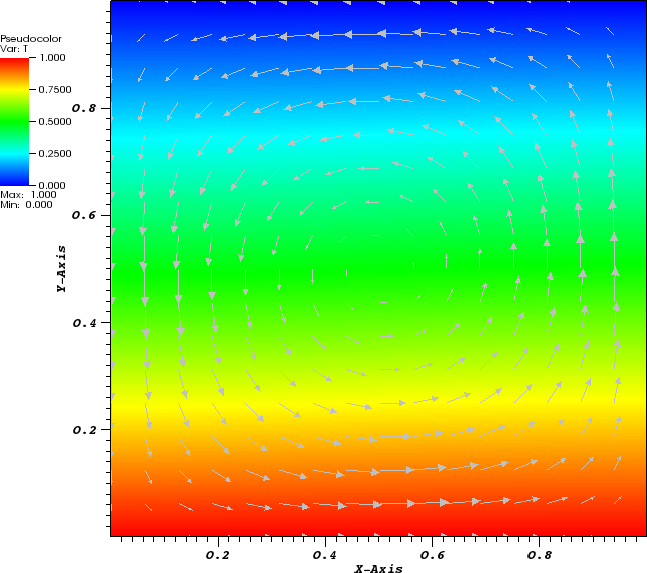
\includegraphics[width=0.4\textwidth]{visit0000.png}
\hfill
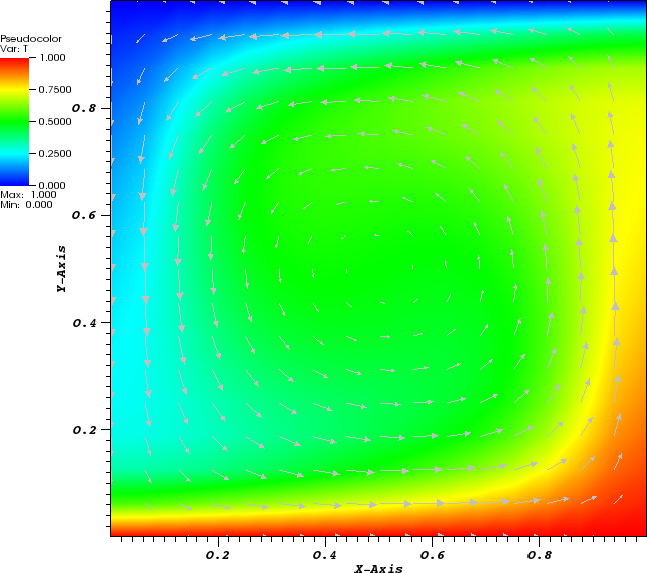
\includegraphics[width=0.4\textwidth]{visit0001.png}
\hfill
\phantom.
\caption{\it Convection in a box: Initial temperature and velocity field (left)
and final state (right).}
\label{fig:convection-box-fields}
\end{figure}

There are many other things we can learn from the output files generated by
\aspect{}, specifically from the statistics file that contains information
collected at every time step and that has been discussed in
Section~\ref{sec:viz-stat}. In particular, in our input file, we have selected
that we would like to compute velocity, temperature, and heat flux statistics.
These statistics, among others, are listed in the statistics file whose head
looks like this for the current input file:
\begin{lstlisting}[frame=single,language=prmfile]
# 1: Time step number
# 2: Time (seconds)
# 3: Time step size (seconds)
# 4: Number of mesh cells
# 5: Number of Stokes degrees of freedom
# 6: Number of temperature degrees of freedom
# 7: Iterations for temperature solver
# 8: Iterations for Stokes solver
# 9: Velocity iterations in Stokes preconditioner
# 10: Schur complement iterations in Stokes preconditioner
# 11: RMS velocity (m/s)
# 12: Max. velocity (m/s)
# 13: Minimal temperature (K)
# 14: Average temperature (K)
# 15: Maximal temperature (K)
# 16: Average nondimensional temperature (K)
# 17: Outward heat flux through boundary with indicator 0 ("left") (W)
# 18: Outward heat flux through boundary with indicator 1 ("right") (W)
# 19: Outward heat flux through boundary with indicator 2 ("bottom") (W)
# 20: Outward heat flux through boundary with indicator 3 ("top") (W)
# 21: Visualization file name
... lots of numbers arranged in columns ...
\end{lstlisting}

Fig.~\ref{fig:convection-box-stats} shows the results of visualizing the data
that can be found in columns 2 (the time) plotted against columns 11 and 12
(root mean square and maximal velocities). Plots of this kind can be generated with
\texttt{Gnuplot} by typing (see Section~\ref{sec:viz-stat} for a more thorough
discussion):
\begin{verbatim}
  plot "output-convection-box/statistics" using 2:11 with lines
\end{verbatim}
Fig.~\ref{fig:convection-box-stats} shows clearly that the simulation
enters a steady state after about $t\approx 0.1$ and then changes very little. This can also be observed using the
graphical output files from which we have generated
Fig.~\ref{fig:convection-box-fields}. One can look further into this data to
find that the flux through the top and bottom boundaries is not exactly the same
(up to the obvious difference in sign, given that at the bottom boundary heat
flows into the domain and at the top boundary out of it) at the beginning of the
simulation until the fluid has attained its equilibrium. However, after
$t\approx 0.2$, the fluxes differ by only $\num{5e-5}$, i.e., by less than
0.001\% of their magnitude.%
\footnote{This difference is far smaller than the numerical error in the heat
flux on the mesh this data is computed on.}
The flux we get at the last time step, 4.787, is less than 2\% away from the
value reported in \cite{BBC89} ($\approx$4.88) although we compute on a $16\times 16$ mesh and
the values reported by Blankenbach are extrapolated from meshes of size up to
$72\times 72$. This shows the accuracy that can be obtained using a higher order
finite element. Secondly, the fluxes through the left and right boundary are not
exactly zero but small. Of course, we have prescribed boundary conditions of the
form $\frac{\partial T}{\partial \mathbf n}=0$ along these boundaries, but this
is subject to discretization errors. It is easy to verify that the heat flux
through these two boundaries disappears as we refine the mesh further.

\begin{figure}
\phantom.
\hfill
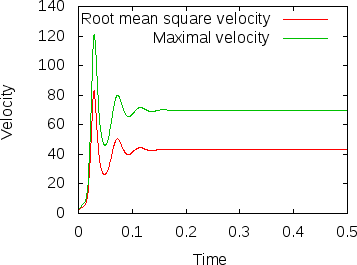
\includegraphics[width=0.4\textwidth]{velocity.png}
\hfill
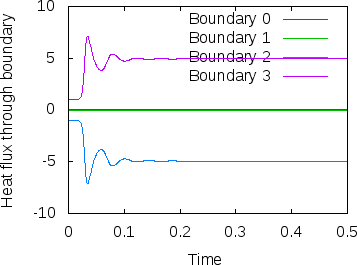
\includegraphics[width=0.4\textwidth]{heatflux.png}
\hfill
\phantom.
\caption{\it Convection in a box: Root mean square and maximal velocity as a
function of simulation time (left). Heat flux through the four boundaries of
the box (right).}
\label{fig:convection-box-stats}
\end{figure}


Furthermore, \aspect{} automatically also collects statistics about many of its
internal workings. Fig.~\ref{fig:convection-box-iterations} shows the number of
iterations required to solve the Stokes and temperature linear systems in each
time step. It is easy to see that these are more difficult to solve in the
beginning when the solution still changes significant from time step to time
step. However, after some time, the solution remains mostly the same and solvers
then only need 9 or 10 iterations for the temperature equation and 4 or 5
iterations for the Stokes equations because the starting guess for the linear
solver -- the previous time step's solution -- is already pretty good. If you
look at any of the more complex cookbooks, you will find that one needs many
more iterations to solve these equations.

\begin{figure}
\phantom.
\hfill
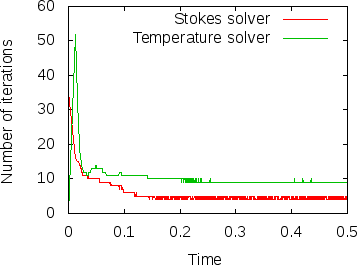
\includegraphics[width=0.4\textwidth]{iterations.png}
\hfill
\phantom.
\caption{\it Convection in a box: Number of linear iterations required to solve
the Stokes and temperature equations in each time step.}
\label{fig:convection-box-iterations}
\end{figure}

\note{If you want to run a version of this cookbook that uses Earth-like rather than nondimensional parameters, and that includes particles that visualize the flow field, see Section~\ref{sec:cookbooks-running-a-model}.}


\paragraph{Play time 1: Different Rayleigh numbers.} After showing you results
for the input file as it can be found in \url{cookbooks/convection-box.prm}, let us
end this section with a few ideas on how to play with it and what to explore.
The first direction one could take this example is certainly to consider
different Rayleigh numbers. As mentioned above, for the value $Ra=10^4$ for
which the results above have been produced, one gets a stable convection
pattern. On the other hand, for values $Ra<Ra_c\approx 780$, any movement of
the fluid dies down exponentially and we end up with a situation where the fluid
doesn't move and heat is transported from the bottom to the top only through
heat conduction. This can be explained by considering that the Rayleigh number
in a box is defined as $Ra=\frac{\rho_0 g\alpha\Delta T h^3}{\eta k}$. A small
Rayleigh number below $Ra_c$ means that the buoyancy forces 
caused by temperature variations 
-- $\rho_0 \alpha \Delta T$ -- are not strong enough to overcome friction forces within the fluid, that is, the viscosity is too high.

On the other hand, if the Rayleigh number is large (i.e., the viscosity is
small or the buoyancy large) then the fluid develops an unsteady convection
period. As we consider fluids with larger and larger $Ra$, this pattern goes
through a sequence of period-doubling events until flow finally becomes chaotic.
The structures of the flow pattern also become smaller and smaller.

\begin{figure}
\phantom.
\hfill
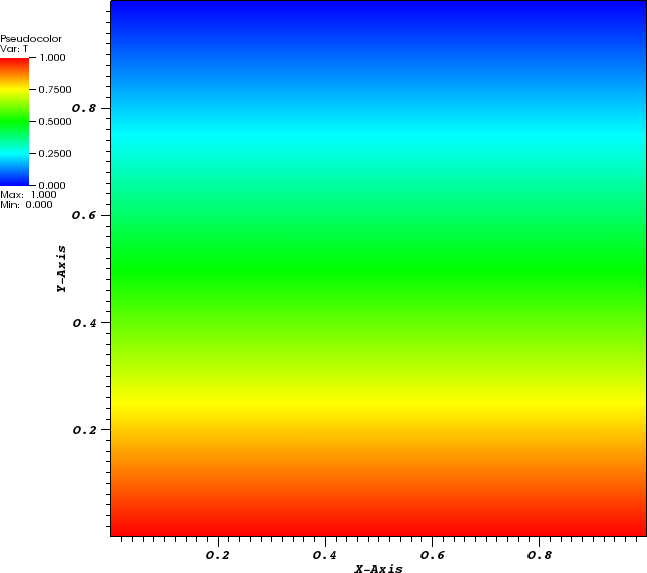
\includegraphics[width=0.4\textwidth]{ra_1e2_visit0000.png}
\hfill
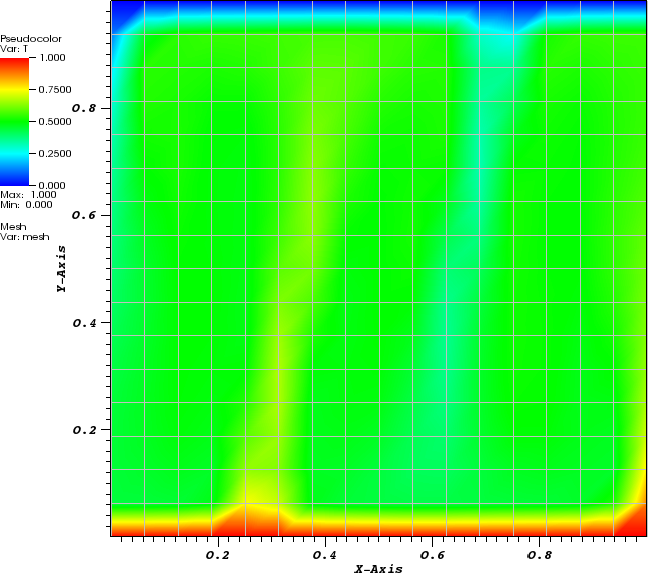
\includegraphics[width=0.4\textwidth]{ra_1e6_visit0001.png}
\hfill
\phantom.
\caption{\it Convection in a box: Temperature fields at the end of a
simulation for $Ra=10^2$ where thermal diffusion dominates (left) and $Ra=10^6$
where convective heat transport dominates (right).
The mesh on the right is clearly too coarse to resolve the structure of the solution.}
\label{fig:convection-box-fields-different-Ra}
\end{figure}

\begin{figure}
\phantom.
\hfill
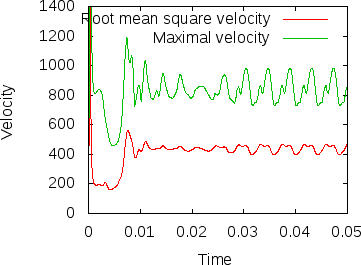
\includegraphics[width=0.4\textwidth]{ra_1e6_velocity.png}
\hfill
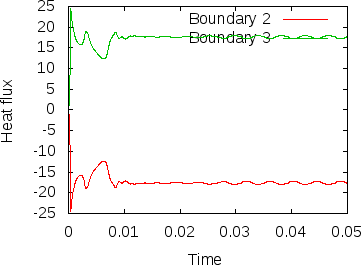
\includegraphics[width=0.4\textwidth]{ra_1e6_heatflux.png}
\hfill
\phantom.
\caption{\it Convection in a box: Velocities (left) and heat flux across the
top and bottom boundaries (right) as a function of time at $Ra=10^6$.}
\label{fig:convection-box-stats-different-Ra}
\end{figure}

We illustrate these situations in
Figs.~\ref{fig:convection-box-fields-different-Ra} and
\ref{fig:convection-box-stats-different-Ra}. The first shows the temperature
field at the end of a simulation for $Ra=10^2$ (below $Ra_c$) and at $Ra=10^6$.
Obviously, for the right picture, the mesh is not fine enough to accurately
resolve the features of the flow field and we would have to refine it more. The
second of the figures shows the velocity and heatflux statistics for the
computation with $Ra=10^6$; it is obvious here that the flow no longer settles
into a steady state but has a periodic behavior. This can also be seen by
looking at movies of the solution.

To generate these results, remember that we have chosen 
$g=Ra$ in our input file. In other words, changing the input file to
contain the parameter setting
%
\lstinputlisting[language=prmfile]{gravity.part.prm.out}
%
will achieve the desired effect of computing with $Ra=10^6$.


\paragraph{Play time 2: Thinking about finer meshes.}
In our computations for $Ra=10^4$ we used a $16\times 16$ mesh and obtained a
value for the heat flux that differed from the generally accepted value from
Blankenbach \textit{et al.} \cite{BBC89} by less than 2\%. However, it may be
interesting to think about computing even more accurately. This is easily done
by using a finer mesh, for example. In the parameter file above, we have chosen
the mesh setting as follows:
%
\lstinputlisting[language=prmfile]{refine.part.prm.out}
%
We start out with a box geometry consisting of a single cell that is refined
four times. Each time we split each cell into its 4 children, obtaining the
$16\times 16$ mesh already mentioned. The other settings indicate that we do not
want to refine the mesh adaptively at all in the first time step, and a setting
of zero for the last parameter means that we also never want to adapt the mesh
again at a later time. Let us stick with the never-changing, globally refined
mesh for now (we will come back to adaptive mesh refinement again at a later
time) and only vary the initial global refinement. In particular, we could
choose the parameter \texttt{Initial global refinement} to be 5, 6, or even
larger. This will get us closer to the exact solution albeit at the expense of a
significantly increased computational time.

A better strategy is to realize that for $Ra=10^4$, the flow enters a steady
state after settling in during the first part of the simulation (see, for
example, the graphs in Fig.~\ref{fig:convection-box-stats}). Since we are not
particularly interested in this initial transient process, there is really no
reason to spend CPU time using a fine mesh and correspondingly small time
steps during this part of the simulation (remember that each refinement results
in four times as many cells in 2d and a time step half as long, making reaching
a particular time at least 8 times as expensive, assuming that all solvers in
\aspect{} scale perfectly with the number of cells). Rather, we can use a
parameter in the \aspect{} input file that let's us increase the mesh resolution
at later times. To this end, let us use the following snippet for the input
file:
\lstinputlisting[language=prmfile]{refine2.part.prm.out}

What this does is the following: We start with an $8\times 8$ mesh (3 times
globally refined) but then at times $t=0.2,0.3$ and $0.4$ we refine the mesh
using the default refinement indicator (which one this is is not important
because of the next statement). Each time, we refine, we refine a fraction 1.0
of the cells, i.e., \textit{all} cells and we coarsen a fraction of 0.0 of the
cells, i.e. no cells at all. In effect, at these additional refinement times, we
do another global refinement, bringing us to refinement levels 4, 5 and finally
6.

\begin{figure}
\phantom.
\hfill
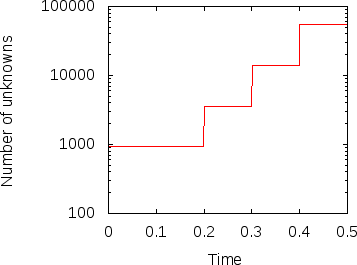
\includegraphics[width=0.4\textwidth]{steps_unknowns.png}
\hfill
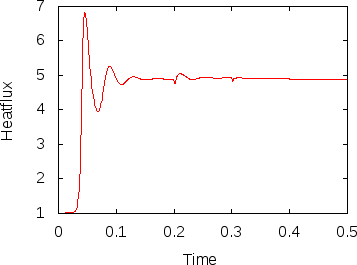
\includegraphics[width=0.4\textwidth]{steps_heatflux.png}
\hfill
\phantom.
\caption{\it Convection in a box: Refinement in stages. Total number
of unknowns in each time step, including all velocity, pressure and
temperature unknowns (left) and heat flux across the top boundary (right).}
\label{fig:convection-box-stats-steps}
\end{figure}


Fig.~\ref{fig:convection-box-stats-steps} shows the results. In the left panel,
we see how the number of unknowns grows over time (note the logscale for the
$y$-axis). The right panel displays the heat flux. The jumps in the number of
cells is clearly visible in this picture as well. This may be surprising at
first but remember that the mesh is clearly too coarse in the beginning to
really resolve the flow and so we should expect that the solution changes
significantly if the mesh is refined. This effect becomes smaller with every
additional refinement and is barely visible at the last time this happens,
indicating that the mesh before this refinement step may already have been fine
enough to resolve the majority of the dynamics.

In any case, we can compare the heat fluxes we obtain at the end of these
computations: With a globally four times refined mesh, we get a value of 4.787
(an error of approximately 2\% against the accepted value from Blankenbach,
$4.884409\pm 0.00001$). With a globally five times refined mesh we get 4.879, 
and with a globally six times refined mesh we get 4.89 (an error of almost 0.1\%).
With the mesh generated using the procedure above we also get
4.89 with the digits printed on the screen%
\footnote{The statistics file gives this
value to more digits: 4.89008498. However, these are clearly more digits than
the result is accurate.}
(also corresponding to an error of almost 0.1\%). In other words, our
simple procedure of refining the mesh during the simulation run yields the same 
accuracy as using the mesh that is globally refined in the beginning of the 
simulation, while needing a much lower compute time.  


\paragraph{Play time 3: Changing the finite element in use.}
Another way to increase the accuracy of a finite element computation is to use a
higher polynomial degree for the finite element shape functions. By default,
\aspect{} uses quadratic shape functions for the velocity and the temperature
and linear ones for the pressure. However, this can be changed with a single
number in the input file.

Before doing so, let us consider some aspects of such a change. First, looking
at the pictures of the solution in Fig.~\ref{fig:convection-box-fields}, one
could surmise that the quadratic elements should be able to resolve the velocity
field reasonably well given that it is rather smooth. On the other hand, the
temperature field has a boundary layer at the top and bottom. One could
conjecture that the temperature polynomial degree is therefore the limiting
factor and not the polynomial degree for the flow variables. We will test this
conjecture below. Secondly, given the nature of the equations, increasing the
polynomial degree of the flow variables increases the cost to solve these
equations by a factor of $\frac{22}{9}$ in 2d (you can get this factor by
counting the number of degrees of freedom uniquely associated with each cell) but leaves
the time step size and the cost of solving the temperature system unchanged. On
the other hand, increasing the polynomial degree of the temperature variable
from 2 to 3 requires $\frac 94$ times as many degrees of freedom for the
temperature and also requires us to reduce the size of the time step by a factor
of $\frac 23$. Because solving the temperature system is not a dominant factor
in each time step (see the timing results shown at the end of the screen output
above), the reduction in time step is the only important factor. Overall,
increasing the polynomial degree of the temperature variable turns out to be the
cheaper of the two options.

Following these considerations, let us add the following section to the
parameter file:
\lstinputlisting[language=prmfile]{disc.part.prm.out}

This leaves the velocity and pressure shape functions at quadratic and linear
polynomial degree but increases the polynomial degree of the temperature from
quadratic to cubic. Using the original, four times globally refined mesh, we
then get the following output:
\begin{lstlisting}[frame=single,language=ksh]
Number of active cells: 256 (on 5 levels)
Number of degrees of freedom: 4,868 (2,178+289+2,401)

*** Timestep 0:  t=0 seconds
   Solving temperature system... 0 iterations.
   Rebuilding Stokes preconditioner...
   Solving Stokes system... 30+0 iterations.

[... ...]

*** Timestep 1621:  t=0.5 seconds
   Solving temperature system... 0 iterations.
   Solving Stokes system... 1+0 iterations.

   Postprocessing:
     RMS, max velocity:                  42.9 m/s, 69.5 m/s
     Temperature min/avg/max:            0 K, 0.5 K, 1 K
     Heat fluxes through boundary parts: -0.004602 W, 0.004602 W, -4.849 W, 4.849 W

Termination requested by criterion: end time


+---------------------------------------------+------------+------------+
| Total wallclock time elapsed since start    |      53.6s |            |
|                                             |            |            |
| Section                         | no. calls |  wall time | % of total |
+---------------------------------+-----------+------------+------------+
| Assemble Stokes system          |      1622 |      4.04s |       7.5% |
| Assemble temperature system     |      1622 |      24.4s |        46% |
| Build Stokes preconditioner     |         1 |    0.0121s |         0% |
| Build temperature preconditioner|      1622 |      8.05s |        15% |
| Solve Stokes system             |      1622 |      8.92s |        17% |
| Solve temperature system        |      1622 |      1.67s |       3.1% |
| Initialization                  |         1 |    0.0327s |         0% |
| Postprocessing                  |      1622 |      4.27s |         8% |
| Setup dof systems               |         1 |   0.00418s |         0% |
| Setup initial conditions        |         1 |   0.00236s |         0% |
+---------------------------------+-----------+------------+------------+

\end{lstlisting}

The heat flux through the top and bottom boundaries is now computed as 4.878.
Using the five times globally refined mesh, it is 4.8837 (an error of 0.015\%). 
This is 6 times more accurate than the 
once more globally refined mesh with the original quadratic elements, at a cost
significantly smaller. Furthermore, we can of course combine this with the mesh
that is gradually refined as simulation time progresses, and we then get a heat
flux that is equal to 4.884446, also only 0.01\% away from the accepted value!

As a final remark, to test our hypothesis that it was indeed the temperature
polynomial degree that was the limiting factor, we can increase the Stokes
polynomial degree to 3 while leaving the temperature polynomial degree at 2. A
quick computation shows that in that case we get a heat flux of 4.747 -- almost 
the same value as we got initially with the lower order Stokes element. In other
words, at least for this testcase, it really was the temperature variable that
limits the accuracy.
